\documentclass[12pt]{article}

\usepackage[brazilian]{babel}
\usepackage[utf8]{inputenc}
\usepackage[T1]{fontenc}
\usepackage{graphicx}
\usepackage{geometry}
\usepackage{booktabs}
\usepackage{float}
\usepackage{longtable}
\usepackage[table]{xcolor}
\usepackage{tcolorbox}
\usepackage{enumitem}
\usepackage{fancyvrb}
\usepackage{hyperref}

\geometry{a4paper, left=3cm, top=3cm, right=2cm, bottom=2cm}
\definecolor{rosa}{HTML}{D6336C}
\hypersetup{colorlinks=true, linkcolor=rosa, urlcolor=rosa}
\setlength{\parindent}{0pt}
\setlength{\parskip}{6pt}

% Caixa de dica / atenção
\newtcolorbox{dica}[1][Dica]{colback=rosa!6, colframe=rosa, title=#1, fonttitle=\bfseries, boxrule=0.6pt}
% Figura padronizada: \figura{arquivo}{legenda}{largura}
\newcommand{\figura}[3]{\begin{figure}[H]\centering\fbox{\includegraphics[width=#3\textwidth]{img/#1}}\caption{#2}\end{figure}}
\newcommand{\botao}[1]{\textbf{[#1]}}

% ------------------------------------------------------------------ CAPA
\begin{document}
\begin{titlepage}
    \centering
    \textsc{\Large Universidade Cruzeiro do Sul}\\[0.5cm]
    \textsc{\Large Engenharia de Software}\\[0.5cm]
    \textsc{Projeto Integrador Transdisciplinar II}
    \vspace{2.5cm}

    \hrule \vspace{0.4cm}
    {\huge \bfseries Manual de Uso\\[0.3cm] Loja Virtual de Cupcakes}\\[0.4cm]
    \hrule
    \vspace{3cm}

    \begin{flushleft}
        \Large \emph{Aluno:}\\
        Fellipe Augusto Gonçalves Magalhães
    \end{flushleft}
    \vfill
    {\large Novembro de 2026}
\end{titlepage}

\tableofcontents
\newpage

% ------------------------------------------------------------------ 1
\section{Apresentação}

Este manual ensina a instalar e a usar a \textbf{Loja Virtual de Cupcakes}, sistema web desenvolvido no Projeto Integrador. Ele é voltado a dois perfis de usuário:

\begin{itemize}
\item \textbf{Cliente:} escolhe cupcakes na vitrine, monta o carrinho, finaliza o pedido, paga e acompanha a entrega.
\item \textbf{Dono da loja (administrador):} cadastra e edita produtos, controla o estoque, atualiza o andamento dos pedidos e consulta as vendas.
\end{itemize}

O sistema é composto por um servidor em Java (padrão MVC), um banco de dados PostgreSQL e telas em HTML, CSS e JavaScript que funcionam em qualquer navegador moderno.

% ------------------------------------------------------------------ 2
\section{Requisitos}

\begin{table}[H]
\centering
\renewcommand{\arraystretch}{1.25}
\begin{tabular}{|l|p{8.5cm}|}
\hline
\rowcolor{gray!30} \textbf{Item} & \textbf{Versão / observação} \\ \hline
Java (JDK) & 17 ou superior. Confira com \texttt{javac -version} \\ \hline
Banco de dados & PostgreSQL 14 ou superior (pode ser em Docker) \\ \hline
Docker (opcional) & Facilita a criação do banco \\ \hline
Navegador & Chrome, Edge ou Firefox atualizados \\ \hline
\end{tabular}
\caption{Requisitos para executar o sistema}
\end{table}

% ------------------------------------------------------------------ 3
\section{Instalação e execução}

\subsection{Criar o banco de dados}

Com o Docker instalado, abra um terminal (Prompt de Comando ou PowerShell) e crie o container do PostgreSQL:

\begin{Verbatim}[fontsize=\footnotesize, frame=single]
docker run -d --name loja-db -e POSTGRES_PASSWORD=postgres ^
  -e POSTGRES_DB=loja_cupcakes -p 5432:5432 postgres:16
\end{Verbatim}

O \texttt{\^{}} no fim da primeira linha continua o comando no Prompt de Comando. No PowerShell, troque-o pelo acento grave (\texttt{`}) ou digite tudo em uma linha só.

Em seguida, dentro da pasta do projeto, carregue as tabelas e os dados de demonstração:

\begin{Verbatim}[fontsize=\footnotesize, frame=single]
docker exec -i loja-db psql -U postgres -d loja_cupcakes < sql\schema_loja_cupcakes.sql
\end{Verbatim}

No PowerShell, o símbolo \texttt{<} não funciona. Use:

\begin{Verbatim}[fontsize=\footnotesize, frame=single]
Get-Content sql\schema_loja_cupcakes.sql -Raw -Encoding UTF8 |
  docker exec -i loja-db psql -U postgres -d loja_cupcakes
\end{Verbatim}

\begin{dica}[Sem Docker]
Se você já tem o PostgreSQL instalado, crie o banco com \texttt{createdb -U postgres loja\_cupcakes} e rode o arquivo SQL com \texttt{psql -U postgres -d loja\_cupcakes -f sql/schema\_loja\_cupcakes.sql}.
\end{dica}

Para parar e religar o banco depois: \texttt{docker stop loja-db} e \texttt{docker start loja-db}. Os dados permanecem enquanto o container não for apagado.

\subsection{Compilar e executar o sistema}

Na pasta do projeto (\texttt{loja-cupcakes}), abra o terminal e execute:

\begin{Verbatim}[fontsize=\footnotesize, frame=single]
compilar.bat
executar.bat
\end{Verbatim}

No PowerShell, coloque \texttt{.\textbackslash} antes do nome (\texttt{.\textbackslash compilar.bat}). No Linux/Mac use \texttt{./compilar.sh} e \texttt{./executar.sh}.

Quando aparecer a mensagem \texttt{Loja de Cupcakes em http://localhost:8080}, o sistema está no ar. \textbf{Mantenha a janela do terminal aberta} enquanto usa a loja. Para encerrar, feche a janela ou tecle \texttt{Ctrl+C}.

\subsection{Configurações opcionais}

Se a senha do banco não for \texttt{postgres} ou se a porta 8080 estiver ocupada, defina variáveis antes de executar:

\begin{table}[H]
\centering
\renewcommand{\arraystretch}{1.25}
\begin{tabular}{|l|p{5.2cm}|p{4.2cm}|}
\hline
\rowcolor{gray!30} \textbf{Variável} & \textbf{Função} & \textbf{Padrão} \\ \hline
\texttt{DB\_PASSWORD} & Senha do banco & \texttt{postgres} \\ \hline
\texttt{DB\_USER} & Usuário do banco & \texttt{postgres} \\ \hline
\texttt{DB\_URL} & Endereço (JDBC) do banco & \texttt{localhost}, porta 5432 \\ \hline
\texttt{PORT} & Porta do site & \texttt{8080} \\ \hline
\end{tabular}
\caption{Variáveis de ambiente}
\end{table}

Exemplos (Prompt de Comando e PowerShell):

\begin{Verbatim}[fontsize=\footnotesize, frame=single]
set DB_PASSWORD=minha_senha
$env:DB_PASSWORD="minha_senha"
\end{Verbatim}

Digite apenas a linha do seu terminal, antes de rodar \texttt{executar.bat}.

\subsection{Contas de demonstração}

\begin{table}[H]
\centering
\renewcommand{\arraystretch}{1.25}
\begin{tabular}{|l|l|l|}
\hline
\rowcolor{gray!30} \textbf{Perfil} & \textbf{E-mail} & \textbf{Senha} \\ \hline
Cliente & maria@email.com & 123456 \\ \hline
Cliente & joao@email.com & 123456 \\ \hline
Administrador & admin@cupcakes.com & 123456 \\ \hline
\end{tabular}
\caption{Contas criadas pelo script do banco}
\end{table}

% ------------------------------------------------------------------ 4
\section{Usando a loja como cliente}

Abra o navegador em \url{http://localhost:8080}.

\subsection{Entrar e criar conta}

Ao abrir o endereço, aparece \textbf{somente a tela de login}. A loja só é mostrada depois que você entra.

\figura{01_login.png}{Tela inicial: somente o login}{0.95}

Para entrar, informe e-mail e senha e clique em \botao{Entrar} (ou tecle Enter). Se os dados estiverem errados, aparece a mensagem ``E-mail ou senha inválidos''.

Para criar uma conta, clique na aba \botao{Criar conta}, preencha nome, e-mail, senha com no mínimo 6 caracteres e, se quiser, o telefone (somente números). Depois de cadastrar, volte à aba \botao{Entrar} e faça o login.

\figura{02_cadastro.png}{Formulário de criação de conta}{0.45}

\subsection{Vitrine e filtro por categoria}

Depois do login, a vitrine mostra os cupcakes disponíveis, com preço e categorias. Os itens em destaque aparecem primeiro.

\figura{03_vitrine.png}{Vitrine de cupcakes}{0.95}

Para filtrar, escolha uma categoria na lista \textbf{Categoria} (por exemplo, \emph{Vegano} ou \emph{Sem lactose}). A lista se atualiza na hora. Escolha \emph{Todas} para voltar a ver tudo.

\figura{04_filtro.png}{Vitrine filtrada pela categoria ``Vegano''}{0.95}

\subsection{Ver detalhes do cupcake}

Clique em \botao{Detalhes} para ver a descrição completa, os ingredientes e o preço. Dessa janela você também pode adicionar o produto ao carrinho.

\figura{05_detalhes.png}{Janela de detalhes do produto}{0.95}

\subsection{Carrinho}

Clique em \botao{Adicionar} para colocar um cupcake no carrinho. Aparece o aviso ``Item adicionado ao carrinho'' e o número ao lado de \botao{Carrinho} no topo da página aumenta. Clicar de novo no mesmo produto soma mais uma unidade.

\figura{06_adicionado.png}{Aviso de item adicionado e contador do carrinho}{0.95}

Para ver o carrinho, clique em \botao{Carrinho} no topo. Ele abre como uma \textbf{aba lateral}, à direita da tela, com os itens, as quantidades, o subtotal de cada um e o total. Para tirar um produto, clique em \botao{Remover}. Para fechar a aba, clique no \botao{X} ou em qualquer ponto fora dela.

\figura{07_carrinho.png}{Aba lateral do carrinho com o botão Finalizar pedido}{0.95}

\subsection{Finalizar o pedido}

\begin{enumerate}
\item Na aba do carrinho, clique em \botao{Finalizar pedido}. O botão fica desabilitado quando o carrinho está vazio.
\item Escolha o endereço de entrega na lista.
\item Se ainda não tiver endereço, ou quiser outro, clique em \botao{+ Novo endereço}, preencha CEP (8 dígitos), rua, número, bairro, cidade e UF, e clique em \botao{Salvar endereço}. O novo endereço já fica selecionado.
\item Clique em \botao{Confirmar pedido}. A taxa de entrega de R\$ 5,00 é somada ao total.
\end{enumerate}

\figura{08_checkout.png}{Janela de finalização: escolha do endereço}{0.95}

\figura{09_novo_endereco.png}{Cadastro de um novo endereço}{0.95}

\begin{dica}[Estoque]
Se algum produto do carrinho não tiver mais unidades suficientes, o pedido não é confirmado e o sistema avisa. Remova o item ou escolha outro.
\end{dica}

\subsection{Pagamento}

Ao confirmar o pedido, abre a janela de pagamento. Escolha \textbf{PIX} ou \textbf{Cartão} e clique em \botao{Pagar}.

\figura{10_pagamento.png}{Janela de pagamento}{0.95}

O pagamento nesta versão é uma \textbf{simulação}: nenhum dado real de cartão é pedido ou guardado. Para demonstrar o que acontece quando o pagamento falha, marque a caixa ``Simular pagamento recusado'' antes de pagar. O sistema avisa que o pagamento foi recusado e você pode tentar de novo.

\begin{figure}[H]
\centering
\fbox{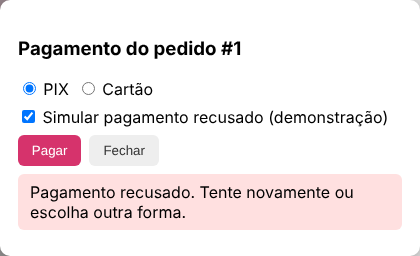
\includegraphics[width=0.46\textwidth]{img/11_recusado.png}}\hfill
\fbox{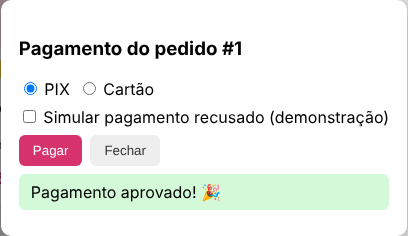
\includegraphics[width=0.46\textwidth]{img/12_aprovado.png}}
\caption{Pagamento recusado (esquerda) e aprovado (direita)}
\end{figure}

Se você fechar a janela sem pagar, o pedido continua aguardando pagamento. Para pagar depois, abra \botao{Meus pedidos} e clique em \botao{Pagar agora}.

\subsection{Meus pedidos}

Clique em \botao{Meus pedidos} no topo (ou na segunda aba da lateral) para acompanhar suas compras. Cada pedido mostra o número, a data, o valor, a situação do pagamento e o status:

\begin{table}[H]
\centering
\renewcommand{\arraystretch}{1.25}
\begin{tabular}{|l|p{8cm}|}
\hline
\rowcolor{gray!30} \textbf{Status} & \textbf{Significado} \\ \hline
AGUARDANDO PAGAMENTO & Pedido criado, falta pagar \\ \hline
PAGO & Pagamento aprovado \\ \hline
EM PREPARO & A loja está preparando os cupcakes \\ \hline
ENVIADO & Pedido saiu para entrega \\ \hline
ENTREGUE & Pedido recebido \\ \hline
CANCELADO & Pedido cancelado pela loja \\ \hline
\end{tabular}
\caption{Status do pedido}
\end{table}

\figura{13_meus_pedidos.png}{Aba lateral ``Meus pedidos''}{0.95}

A lista é atualizada sozinha a cada 15 segundos enquanto a aba lateral está aberta.

\subsection{Sair}

Clique em \botao{Sair} no topo para encerrar a sessão. Se a aba lateral estiver aberta, feche-a antes.

% ------------------------------------------------------------------ 5
\section{Usando o painel do dono}

\subsection{Acessar o painel}

Na tela de login, entre com a conta de administrador (\texttt{admin@cupcakes.com}). O sistema leva você direto ao \textbf{painel do dono}. Contas de cliente não têm acesso a essa área.

\subsection{Dashboard de vendas}

No topo do painel ficam três tabelas:
\begin{itemize}
\item \textbf{Vendas por dia:} quantidade de pedidos, faturamento e ticket médio. Contam pedidos já pagos; os aguardando pagamento ou cancelados ficam de fora.
\item \textbf{Mais vendidos:} unidades vendidas e receita por produto.
\item \textbf{Estoque:} unidades de cada produto e sua situação: \textbf{OK}, \textbf{BAIXO} (5 unidades ou menos) ou \textbf{ESGOTADO}.
\end{itemize}

\figura{14_dashboard.png}{Dashboard de vendas}{0.95}

\subsection{Atualizar o status dos pedidos}

Na seção \textbf{Pedidos}, cada linha tem uma lista de status. Escolha o novo status e a alteração é salva na hora, com a mensagem ``Status do pedido atualizado''.

\figura{15_admin_pedidos.png}{Lista de pedidos com troca de status}{0.95}

O sistema só aceita a sequência correta:

\begin{center}
AGUARDANDO PAGAMENTO $\rightarrow$ PAGO $\rightarrow$ EM PREPARO $\rightarrow$ ENVIADO $\rightarrow$ ENTREGUE
\end{center}

Um pedido pode ser cancelado enquanto estiver aguardando pagamento, pago ou em preparo. Pular etapas (por exemplo, de PAGO direto para ENTREGUE) gera a mensagem ``Transição de status inválida''. O status PAGO é definido automaticamente quando o pagamento é aprovado.

\subsection{Cadastrar um novo cupcake}

Na seção \textbf{Novo cupcake}, preencha:

\begin{itemize}
\item \textbf{Nome} (único) e \textbf{descrição}: obrigatórios;
\item \textbf{Preço}: maior que zero;
\item \textbf{Estoque}: quantidade inicial;
\item \textbf{Ingredientes} e \textbf{URL da imagem}: opcionais (sem imagem, aparece um cupcake desenhado);
\item \textbf{Categorias}: marque uma ou mais;
\item \textbf{Destaque}: o produto aparece no início da vitrine;
\item \textbf{Ativo}: só produtos ativos aparecem para os clientes.
\end{itemize}

Clique em \botao{Salvar}. O produto aparece na tabela de produtos cadastrados e, se estiver ativo, na vitrine.

\figura{16_admin_cadastro.png}{Formulário de cadastro de produto}{0.95}

\figura{17_admin_produtos.png}{Produtos cadastrados}{0.95}

\subsection{Editar produto, alterar preço e tirar da vitrine}

Na tabela de produtos, clique em \botao{Editar}. Os dados vão para o formulário, que passa a se chamar ``Editar cupcake''. Altere o que precisar e clique em \botao{Salvar}. Para tirar um produto da vitrine sem apagá-lo, desmarque \textbf{Ativo}. Pedidos antigos continuam mostrando o preço pago na época. Para desistir da edição, clique em \botao{Limpar}.

\subsection{Repor o estoque}

O estoque diminui automaticamente a cada pedido confirmado. Para dar entrada de novas unidades:

\begin{enumerate}
\item Na tabela de produtos, clique em \botao{Editar} no cupcake.
\item No campo \textbf{Estoque}, digite o \textbf{novo total}. Exemplo: se há 4 unidades e chegaram 20, digite 24.
\item Clique em \botao{Salvar}.
\end{enumerate}

\figura{18_admin_editar.png}{Edição de um produto para repor o estoque}{0.95}

\begin{dica}[Atenção]
O campo Estoque recebe o total, e não a quantidade que chegou. O sistema ainda não guarda o histórico das entradas.
\end{dica}

% ------------------------------------------------------------------ 6
\section{Mensagens comuns e solução de problemas}

\begin{longtable}{|p{5.2cm}|p{8.3cm}|}
\hline
\rowcolor{gray!30} \textbf{Mensagem ou sintoma} & \textbf{O que fazer} \\ \hline
\endhead
E-mail ou senha inválidos & Confira os dados. Nas contas de demonstração a senha é 123456 \\ \hline
E-mail já cadastrado & Use outro e-mail ou faça login com o existente \\ \hline
A senha deve ter ao menos 6 caracteres & Escolha uma senha maior \\ \hline
CEP deve ter 8 dígitos & Digite o CEP completo; hífen e pontos são ignorados \\ \hline
Preencha rua, número, bairro e cidade & Todos esses campos do endereço são obrigatórios \\ \hline
Há item inativo ou sem estoque suficiente & Algum produto acabou ou saiu da vitrine; remova-o do carrinho \\ \hline
Faça login para continuar & A sessão expirou (ocorre ao reiniciar o servidor); entre de novo \\ \hline
Transição de status inválida & Siga a ordem do fluxo de status (seção 5.3) \\ \hline
Nome já existe (produto) & Cada cupcake precisa de um nome único \\ \hline
A página não abre & Confira se o terminal do sistema está aberto e mostra a mensagem \texttt{Loja de Cupcakes em ...} \\ \hline
Erro no banco de dados / não conecta & Verifique se o container está ligado (\texttt{docker start loja-db}) e se a senha do banco confere com \texttt{DB\_PASSWORD} \\ \hline
\texttt{'javac' não é reconhecido} & O JDK não está instalado ou não está no PATH. Instale-o e abra um terminal novo \\ \hline
Porta 8080 em uso & Defina outra porta com \texttt{set PORT=8081} e abra \texttt{http://localhost:8081} \\ \hline
\end{longtable}

% ------------------------------------------------------------------ 7
\section{Limitações desta versão}

\begin{itemize}
\item O pagamento é simulado, sem integração com um gateway real.
\item O endereço é digitado pelo cliente; não há consulta automática de CEP.
\item O botão Adicionar insere uma unidade por clique; a quantidade final se ajusta clicando novamente.
\item O painel do dono mostra o dashboard em tabelas, sem gráficos.
\item O status do pedido é atualizado por consulta periódica (15 segundos), e não em tempo real.
\item Cancelar um pedido não devolve as unidades ao estoque; ajuste o estoque manualmente (seção 5.6).
\item As sessões ficam na memória do servidor: ao reiniciá-lo, todos precisam entrar de novo.
\item A conta do administrador é criada pelo script do banco; não há tela para criar outros administradores.
\end{itemize}

\end{document}
